\documentclass[twoside]{article}
\usepackage{aistats2016}

\usepackage{booktabs}
\usepackage{natbib}

\usepackage{hyperref}
%\usepackage[demo]{graphicx}
%\usepackage{subcaption}
\usepackage{url}
\usepackage[utf8x]{inputenc}
\usepackage[english]{babel}
\usepackage{natbib}
\usepackage{nicefrac}
\usepackage{algorithm}
\usepackage{algorithmic}
\usepackage{amsfonts}
\usepackage{graphics}
\usepackage{graphicx}
\usepackage{tikz}
\usepackage{color,soul,amsmath}
\usepackage{amssymb}
\usetikzlibrary{bayesnet}
\tikzstyle{connect}=[-latex]
\tikzstyle{allconnected}=[line width=0.1cm]

%\usepackage{verbatim}
%\usepackage[active,tightpage]{preview}
%\PreviewEnvironment{tikzpicture}
%\usepackage{savetrees}

\def\bbbr{{\rm I\!R}}
\newcommand{\vp}{\vec{\phi}}
\newcommand{\vmu}{\vec{\mu}}
\newcommand{\vf}{\vec{f}}

\newcommand{\I}{\mathcal{I}}


\newcommand{\ud}{\mathrm{d}}
\newcommand{\E}{\mathbb{E}}
\newcommand{\Var}{\mathbb{Var}}
\newcommand{\Cov}{\mathbb{Cov}} 
\newcommand{\vm}{\vec{m}}
\newcommand{\vx}{\vec{x}}
\newcommand{\vr}{\vec{r}}
\newcommand{\vy}{\vec{y}}
\newcommand{\vz}{\vec{z}}
\newcommand{\vY}{\vec{Y}}
\newcommand{\vX}{\vec{X}}
\newcommand{\bx}{\textbf{x}}
\newcommand{\bX}{\textbf{X}}
\newcommand{\bY}{\textbf{Y}}
\newcommand{\bz}{\textbf{z}}
\newcommand{\bw}{\textbf{w}}
\newcommand{\by}{\textbf{y}}
\newcommand{\bL}{\textbf{L}}
\newcommand{\bI}{\textbf{I}}
\newcommand{\vk}{\vec{k}}
\newcommand{\vL}{\vec{\Lambda}}
\newcommand{\xmin}{x_{\min}}
\newcommand{\pmin}{p_{\min}}
\newcommand{\fmin}{f_{\min}}
\newcommand{\hpmin}{\hat{p}_{\min}}
\newcommand{\hqmin}{\hat{q}_{\min}}
\newcommand{\pfmin}{p_{f_{\min}}}
\renewcommand{\vec}{\boldsymbol}
\newcommand{\fun}[1]{\mathsf{#1}}
\renewcommand{\O}{\mathcal{O}}
\newcommand{\GP}{\mathcal{GP}}
\newcommand{\N}{\mathcal{N}}
\newcommand{\Id}{\vec{I}}
\newcommand{\II}{\mathbb{I}}
\newcommand{\future}{\mathcal{F}}
\newcommand{\IR}{\mathbb{R}}
\newcommand{\bk}{\textbf{k}}
\newcommand{\bK}{\textbf{K}}
\newcommand{\tr}{\operatorname{tr}}
\newcommand{\argmin}{\operatorname*{arg\: min}}
\newcommand{\argmax}{\operatorname*{arg\: max}}
\newcommand{\chol}{\operatorname{\mathsf{C}}}

\newcommand{\data}{\mathcal{D}}
\newcommand{\reals}{\mathbb{R}}
\newcommand{\sX}{\mathcal{X}}
\newcommand{\xst}{x_{\ast}}
\newcommand{\yst}{y_{\ast}}

\usepackage{xspace}
\newcommand{\acr}[1]{\textsc{#1}\xspace}
\newcommand{\gp}{\acr{gp}}
\newcommand{\dpp}{\acr{dpp}}
\newcommand{\us}{\acr{glasses}}

\newtheorem{theorem}{Theorem}
\newtheorem{lemma}{Lemma}
\newtheorem{corollary}{Corollary}
\newtheorem{proposition}{Proposition}
\newtheorem{definition}{Definition}
\newtheorem{proof}{Proof}
\newtheorem{conjecture}{Conjecture}

\newcommand*{\addheight}[2][.5ex]{%
  \raisebox{0pt}[\dimexpr\height+(#1)\relax]{#2}%
}


\graphicspath{{./},{./diagrams/}}

% If your paper is accepted, change the options for the package
% aistats2016 as follows:
%
%\usepackage[accepted]{aistats2016}
%
% This option will print headings for the title of your paper and
% headings for the authors names, plus a copyright note at the end of
% the first column of the first page.


\begin{document}

% If your paper is accepted and the title of your paper is very long,
% the style will print as headings an error message. Use the following
% command to supply a shorter title of your paper so that it can be
% used as headings.
%
%\runningtitle{I use this title instead because the last one was very long}

% If your paper is accepted and the number of authors is large, the
% style will print as headings an error message. Use the following
% command to supply a shorter version of the authors names so that
% they can be used as headings (for example, use only the surnames)
%
%\runningauthor{Surname 1, Surname 2, Surname 3, ...., Surname n}

\twocolumn[

\aistatstitle{GLASSES: Relieving The Myopia Of Bayesian Optimisation}

\aistatsauthor{ Anonymous Author 1 \And Anonymous Author 2 \And Anonymous Author 3 }

\aistatsaddress{ Unknown Institution 1 \And Unknown Institution 2 \And Unknown Institution 3 } ]

\begin{abstract}
    We present \us: Global optimisation with Look-Ahead through Stochastic Simulation and Expected-loss Search. 
    The majority of global optimisation approaches in use are myopic, in only considering the impact of the next function value; the non-myopic approaches that do exist are able to consider only a handful of future evaluations. 
    Our novel algorithm, \us, permits the consideration of dozens of evaluations into the future. 
    We show that the far-horizon planning thus enabled leads to substantive performance gains in empirical tests. 
\end{abstract}
\section{Introduction} % (fold)
\label{sec:introduction}

Global optimisation is core to any complex problem where design and choice play a role. 
Within Machine Learning, such problems are found in the tuning of hyperparameters \citep{Snoek*Larochelle*Adams_2012}, sensor selection \citep{Garnett*Osborne*Roberts_2010} or experimental design \citep{martinez-cantin_bayesian_2009}. 
Most global optimisation techniques are myopic, in considering no more than a single step into the future. 
Relieving this myopia requires solving the \emph{multi-step lookahead} problem: the global optimisation of an function by considering the significance of the next function evaluation on function evaluations (steps) further into the future. 
It is clear that a solution to the problem would offer performance gains.
For example, consider the case in which we have a budget of two evaluations with which to optimise a function $f(x)$ over the domain $\sX = [0, 1] \subset \reals$. 
If we are strictly myopic, our first evaluation will likely be at 
$x=\nicefrac{1}{2}$, and our second then at only one of $x=\nicefrac{1}{4}$ and $x=\nicefrac{3}{4}$. 
This myopic strategy will thereby result in ignoring half of the domain $\sX$, regardless of the second choice. 
If we adopt a two-step lookahead approach, we will select function evaluations that will be more evenly distributed across the domain by the time the budget is exhausted. 
We will consequently be better informed about $f$ and its optimum.

There is a limited literature on the multi-step lookahead problem.
\cite{osborne_gaussian_2009} perform multi-step lookahead by optimising future evaluation locations, and sampling over future function values. 
This approach scales poorly with the number of future evaluations considered, and the authors present results for no more than two-step lookahead.
\citep{Marchant*Ramos*Sanner*2014} reframe the multi-step lookahead problem as a partially observed Markov decision process, and adopt a Monte Carlo tree search approach in solving it. 
Again, the scaling of the approach permits the authors to consider no more than six steps into the future. In the past, the multi-step look ahead problem was studied by \cite{StreltsovVakili1999} proposing a utility function that is provably a globally optimal in cases where the model of the function values remains unchanged.

Interestingly, there exists a link between the multi-step lookahead problem and \emph{batch} Bayesian optimisation \citep{Ginsbourger2009,Azimi2011,Azimi2012}. In this later case, batches of locations rather than individual observations are selected in each iteration of the algorithm and evaluated in parallel. When such locations are selected \emph{greedily}, that is, one after the other, the key to selecting good batches relies on the ability of the batch criterion of predicting future steps of the algorithm. In this work we will exploit this parallelism to compute a non-myopic loss for Bayesian optimisation. Our algorithm, \us, provides scaling superior to existing alternatives, which is tested in a variety of experiments. In Section \ref{sec:background} we formalise the problem and describe the contributions of this work. Section \ref{sec:glasses} describe the details of the proposed algorithm. Section \ref{sec:experiments} illustrate the superior performance of \us and we conclude in Section \ref{sec:conclusions} with a discussion about the most interesting results observed in this work.


\section{Background and challenge}\label{sec:background}
\subsection{Bayesian Optimisation with one step look-ahead} % (fold)
\label{sec:bayesian_optimisation}


Let $f: {\mathcal X} \to \bbbr$ be well behaved function defined on a compact subset ${\mathcal X} \subseteq \bbbr^d$. We are interested in solving the global optimization problem of finding 
$$\bx_{M} = \arg \min_{\bx \in {\mathcal X}} f(\bx).$$ 
We assume that $f$ is a \emph{black-box} from which only perturbed evaluations of the type $y_i = f(\bx_i) + \epsilon_i$, with $\epsilon_i \sim\mathcal{N}(0,\sigma^2)$, are  available. Bayesian Optimization is an heuristic strategy to make a series of evaluations $\bx_1,\dots,\bx_n$ of $f$, typically very limited in number,  such that the the minimum of $f$ is evaluated as soon as possible \citep{Lizotte_2008,Jones_2001,Snoek*Larochelle*Adams_2012,Brochu*Cora*DeFreitas_2010}.

Assume that $n$ points have been gathered so far, having a dataset $\data_0 = \{(\bx_i,y_i)\}_{i=1}^N = (\bX_0,\bY_0)$. Before collecting any new point, a surrogate probabilistic model for $f$ is calculated. This is topically a Gaussian Process (GP) $p(f) = \mathcal{GP}(\mu; k)$ with mean function $\mu$ and a covariance function $k$, and whose parameters will be denoted by $\theta$.  Let $\I_0$ be the current available information: the conjunction of $\data_0$, the model parameters and the model likelihood type.  Under Gaussian likelihoods, the predictive distribution for $y_*$ at $\bx_*$ is also Gaussian with mean posterior mean and variance
$$\mu(\bx_{*}|\I_0) = \bk_{\theta}(\bx_*)^\top[\bK_{\theta} + \sigma^2 \textbf{I}]^{-1}\by \mbox{ and}$$
$$\sigma^2(\bx_*|\I_0)=k_{\theta}(\bx_*,\bx_*)-\bk_{\theta}(\bx_*)^\top[\bK_{\theta}+\sigma^2 \textbf{I}]^{-1}\bk_{\theta}(\bx_*),$$
where $\bK_{\theta}$ is the matrix such that $(\bK_{\theta})_{ij}=k_{\theta}(\bx_i,\bx_j)$,  $\bk_{\theta}(\bx_{*}) = [k_{\theta}(\bx_1,\bx_{*}),\dots,k_{\theta}(\bx_n,\bx_{*})]^\top$ \citep{Rasmussen:2005:GPM:1162254}.  


Given the GP model, we now need to determine the best location to sample. Imagine that we only have one remaining evaluation ($n=1$) before we need to report our inferred location about the minimum of $f$. Denote by $\eta = \min \{\bY_0\}$, the current best found value. We can define the loss of evaluating $f$ this last time at $\bx_*$ assuming it is returning $y_*$ as
$$\lambda(y_*)\triangleq \left\{ \begin{array}{lcl}
y_*;             & \mbox{if}  &  y_* \leq \eta \\
 \eta; & \mbox{if}  & y_* > \eta. \\
\end{array}
\right.$$
Therefore the loss corresponds is the new observed minimum, $\min (\eta,y_*)$. Its expectation is 
$$\ \Lambda_1(\bx_*| \I_0) \triangleq \E[ \min (y_*,\eta)]= \int \lambda(y_*)p(y_* |\bx_*,\I_0)\ud y_*$$
where the subscript in $\Lambda$ refers to the fact that we are considering one future evaluations.  Giving the properties of the GP, $\Lambda_1(\bx_*| \I_0)$ can be computed in closed form for any $\bx_* \in \mathcal{X}$. In particular, for $\Phi$ the usual Gaussian cumulative distribution function, we have that
\begin{eqnarray}\label{eq:expected_myopic_loss}
\Lambda_1(\bx_*| \I_0) &  \triangleq & \eta \int_{\eta}^{\infty} \mathcal{N}(y_*;\mu,\sigma^2) \ud y_* \\ \nonumber
& +  & \int_{-\infty}^{\eta} y_* \mathcal{N}(y_*;\mu,\sigma^2) \ud y_*  \\ \nonumber
& = &  \eta +(\mu  - \eta) \Phi (\eta ; \mu, \sigma^2) - \sigma^2 \mathcal{N} (\eta, \mu, \sigma^2), \nonumber
\end{eqnarray}

where we have abbreviated $\sigma^2(y_*|\I_0)$ as $\sigma^2$ and $\mu(y_{*}|\I_0)$ as $\mu$. Finally, the next evaluation is located   where $\Lambda_1(\bx_*| \I_0) $ gives the minimum value. This point can  be obtained by any gradient descent algorithm since analytical expressions for the gradient and Hessian of $\Lambda_1(\bx_*| \I_0)$  exist \citep{osborne_bayesian_2010}. 



% section bayesian_optimisation (end)

% section introduction (end)

\begin{figure*}[t!]
\centering
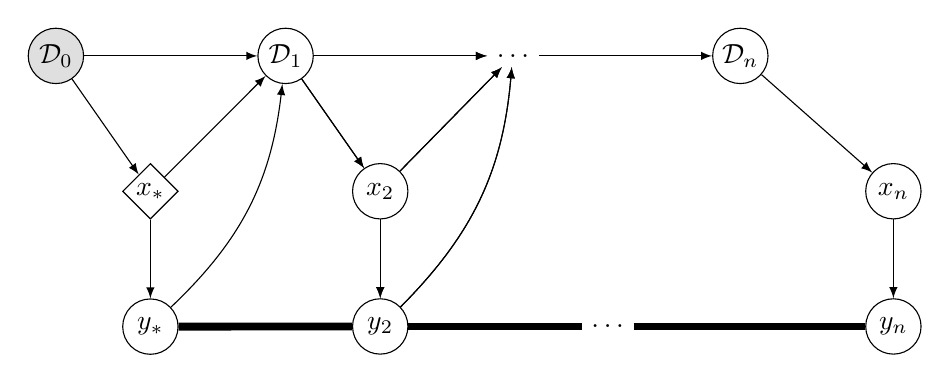
\begin{tikzpicture}

    % first row
    \node[obs] (D0) {$\data_0$};
    \node[latent, right=of D0, xshift=1.2cm] (D1) {$\data_1$};
    \node[draw=none, right=of D1, xshift=1.2cm] (Ddots) {$\ldots$};
    \node[latent, right=of Ddots, xshift=1.2cm] (Dn) {$\data_n$};

    % second row
    \node[det, below=of D0, xshift=1.2cm] (xst) {$\xst$};
    \node[latent, right=of xst, xshift=1.2cm] (x2) {$x_2$};
    \node[latent, right=of x2, xshift=4.8cm] (xn) {$x_n$};

    % third row
    \node[latent, below=of xst] (yst) {$\yst$};
    \node[latent, below=of x2] (y2) {$y_2$};
    \node[draw=none, right=of y2, xshift=1.2cm] (ydots) {$\ldots$};
    \node[latent, below=of xn] (yn) {$y_n$};

    % Connect the nodes
    \path 
        (D0) edge [connect] (D1)
        (D0) edge [connect] (xst)
        (xst) edge [connect] (yst)
        (xst) edge [connect] (D1)
        (yst) edge [connect, bend right=20] (D1)
        (yst) edge [allconnected] (y2)

        (D1) edge [connect] (Ddots)
        (D1) edge [connect] (x2)
        (x2) edge [connect] (y2)
        (x2) edge [connect] (Ddots)
        (y2) edge [connect, bend right=20] (Ddots)
        (y2) edge [allconnected] (ydots)

        (D1) edge [connect] (Ddots)
        (D1) edge [connect] (x2)
        (x2) edge [connect] (y2)
        (x2) edge [connect] (Ddots)
        (y2) edge [connect, bend right=20] (Ddots)
        (ydots) edge [allconnected] (yn)

        (Ddots) edge [connect] (Dn)
        (Dn) edge [connect] (xn)
        (xn) edge [connect] (yn)        
        ;
\end{tikzpicture}
\caption{
    A Bayesian network describing the $n$-step lookahead problem. The shaded node ($\data_0$) is known, and the diamond node ($\xst$) is the current decision variable. All $y$ nodes are correlated with one another under the \gp model.
}
\label{fig:bayes_net}
\end{figure*}

\begin{figure*}[t!]
\centering
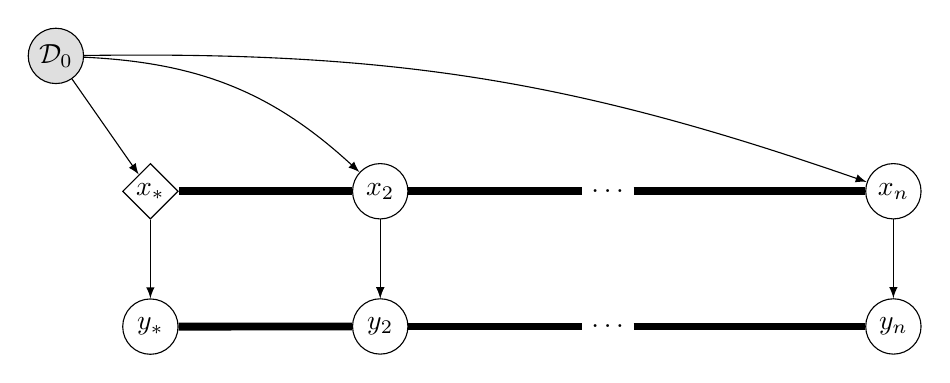
\begin{tikzpicture}

    % first row
    \node[obs] (D0) {$\data_0$};

    % second row
    \node[det, below=of D0, xshift=1.2cm] (xst) {$\xst$};
    \node[latent, right=of xst, xshift=1.2cm] (x2) {$x_2$};
    \node[draw=none, right=of x2, xshift=1.2cm] (xdots) {$\ldots$};
    \node[latent, right=of x2, xshift=4.8cm] (xn) {$x_n$};

    % third row
    \node[latent, below=of xst] (yst) {$\yst$};
    \node[latent, below=of x2] (y2) {$y_2$};
    \node[draw=none, right=of y2, xshift=1.2cm] (ydots) {$\ldots$};
    \node[latent, below=of xn] (yn) {$y_n$};

    % Connect the nodes
    \path 
        (D0) edge [connect] (xst)
        (xst) edge [connect] (yst)
        (yst) edge [allconnected] (y2)

        (D0) edge [connect, bend left=20] (x2)
        (D0) edge [connect, bend left=10] (xn)

        (xst) edge [allconnected] (x2)
        (x2) edge [allconnected] (x2)
        (x2) edge [allconnected] (xdots)
        (xdots) edge [allconnected] (xn)

        (x2) edge [connect] (y2)
        (y2) edge [allconnected] (ydots)

        (x2) edge [connect] (y2)
        (ydots) edge [allconnected] (yn)

        (xn) edge [connect] (yn)        
        ;
\end{tikzpicture}
\caption{
    A Bayesian network describing our approximation to the $n$-step lookahead problem. The shaded node ($\data_0$) is known, and the diamond node ($\xst$) is the current decision variable, which is now directly connected with all future steps of the algorithm.
}
\label{fig:bayes_net_glasses}
\end{figure*}


\subsection{Looking many steps ahead}
Expression~(\ref{eq:expected_myopic_loss}) can also be used as a myopic approximation to the optimal decision when $n$ evaluations of $f$ remain available. Indeed, most BO methods are myopic and ignore the future decisions that will be made by the algorithm in the future steps. 

Denote by $\{(\bx_j,y_j)\}$ for $j=1,\dots,n$ the remaining $n$ available evaluations and by $\I_j$ the available information after the data set $\data_0$ has been augmented with $(\bx_j,y_j),\dots,(\bx_j,y_j)$ and the parameters $\theta$ of the model updated. We use $\Lambda_n(\bx_*|\I_0 )$ to denote the expected loss of selecting $\bx_*$ given $\I_0$ and  considering $n$ future evaluations.  A Proper Bayesian formulation allows us to define this \emph{long-sight} loss  \citep{osborne_bayesian_2010}  as 
\begin{eqnarray}\nonumber
\Lambda_n(\bx_*|\I_0 ) &= & \int \lambda(y_n) \prod_{j=1}^{n}p(y_{j}|\bx_{j},\I_{j-1}) p(\bx_{j}|\I_{j-1})\\\label{eq:expected_nonmyopic_loss}
& & \ud y_*\dots \ud y_n \ud\bx_2\dots \ud\bx_n\footnote{We assume that $p(\bx_*|\I_0)=1$}
\end{eqnarray}
where 
$$p(y_{j}|\bx_{j},\I_{j-1})= \mathcal{N} \left(y_{j};\mu(\bx_{j};\I_{j-1}),\sigma^2(\bx_{j}|\I_{j-1} ) \right)$$ 
is the predictive distribution of the GP at $\bx_{j}$  and 
$$p(\bx_{j}|\I_{j-1}) = \delta (\bx_{j} - \arg \min_{\bx_* \in {\mathcal X}} \Lambda_{n-j+1}(\bx_*|\I_{j-1}))$$ 
reflects the optimization step required to obtain $\bx_{j}$ after all previous the evaluations $f$ have been iteratively optimized and marginalized.  The graphical probabilistic model underlying (\ref{eq:expected_nonmyopic_loss}) is illustrated in Figure \ref{fig:bayes_net}.

To evaluate Eq.~(\ref{eq:expected_nonmyopic_loss}) we can successively sample from $y_1$ to $y_{j-1}$ and optimize for the appropriate $\Lambda_{n-j+1}(\bx_*|\I_{j-1})$. This is in done in \citep{osborne_bayesian_2010} for only two steps look ahead given the computational burden required to compute this loss for longer horizons. Note that analytical expression are only available in the myopic case $\Lambda_1(\bx_*| \I_0)$.

\subsection{Contributions of this work}

The goal of this work is \emph{to propose an efficient approximation to Eq.~(\ref{eq:expected_nonmyopic_loss}) that will relieve the myopia of classical Bayesian optimization}. The precise contributions of this paper are:

\begin{itemize}
\item A new algorithm, \us, to relieve the myopia of Bayesian optimisation that is able to efficiently take into account dozens of steps ahead. The method is based on the prediction of the future steps of the myopic algorithm to efficiently integrate out a long-side loss. 
\item The key aspect of our approach is to split the recursive optimization marginalization loop in Eq.~(\ref{eq:expected_nonmyopic_loss}) into two independent optimisation-marginalization steps that jointly act on all the future steps. We propose an Expectation-Propagation formulation for the joint marginalisation and we discuss different strategies to carry out the optimisation step.
\item Together with this work, we deliver a \emph{open source Python code framework} (link removed for blind review) containing a fully functional  implementation of the method useful to reproduce the results of this work and applicable in general global optimisation problems. As we mentioned in the introduction of this work, there exist a limited literature in BO non-myopic methods and, to our knowledge, no BO package has any myopic loss functions among the available acquisition functions. 
\item Simulations: New practical experiments and insights that show that non-myopic methods outperform myopic approaches in a benchmark of optimisation problems. 
\end{itemize}



\begin{table*}[t!]
\begin{tabular}{ccc}
      \addheight{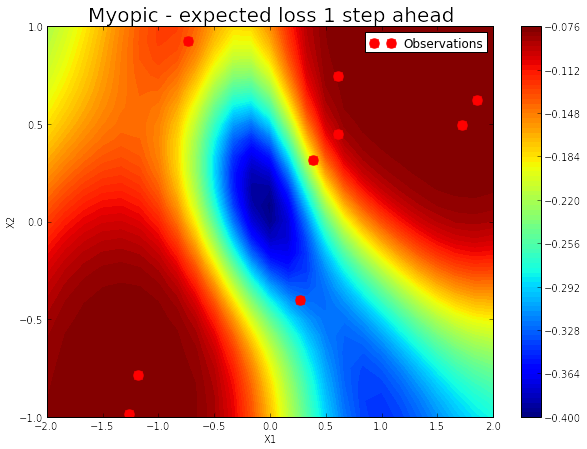
\includegraphics[width=54mm]{bo_1step.png}} &
      \addheight{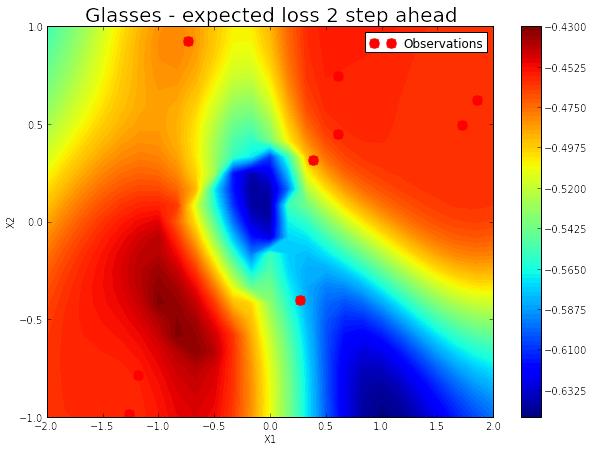
\includegraphics[width=54mm]{bo_2steps.png}}  &
      \addheight{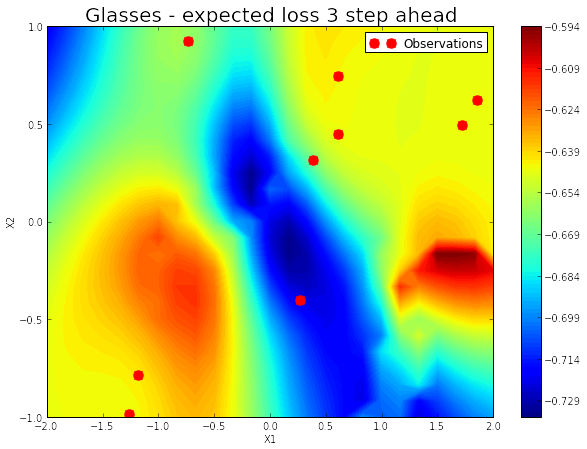
\includegraphics[width=54mm]{bo_3steps.png}}\\
      \small \textbf{Myopic loss} &  \small \textbf{loss 2 steps ahead} & \small \textbf{loss 3 steps ahead} \\
      \addheight{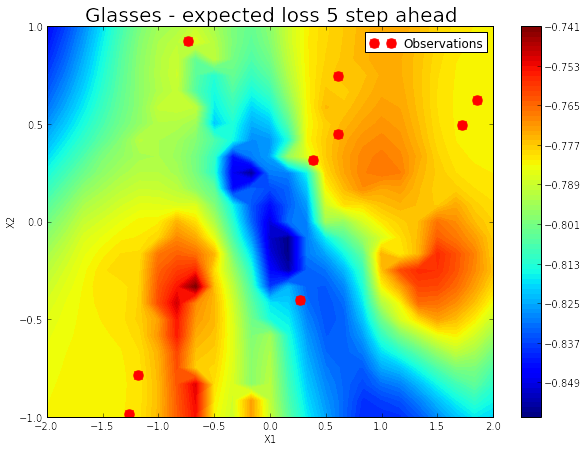
\includegraphics[width=54mm]{bo_5steps.png}} &
      \addheight{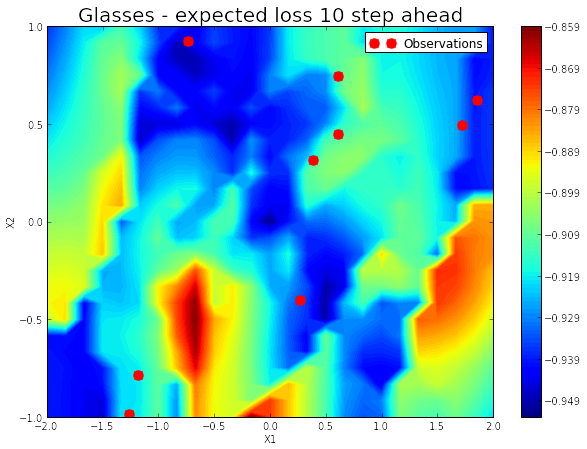
\includegraphics[width=54mm]{bo_10steps.png}}  &
      \addheight{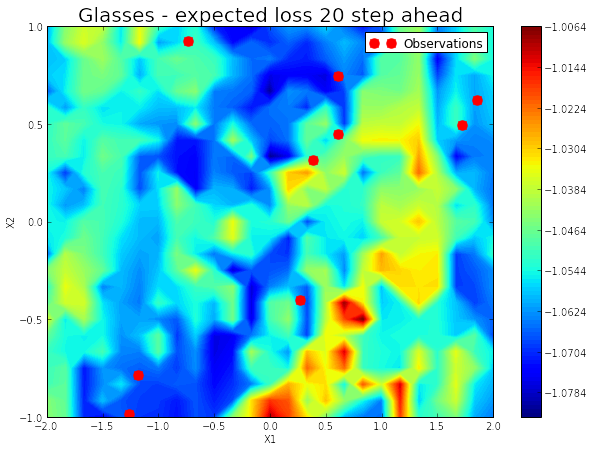
\includegraphics[width=54mm]{bo_20steps.png}}\\
      \small \small \textbf{5 steps ahead} & \small \textbf{10 steps ahead} & \small \textbf{20 steps ahead} \\
\end{tabular}\caption{Estimated expected loss for different number of steps ahead in an example with 10 data points and the Six-hump Camel function. Increasing the steps ahead decreases global optimum of the loss; the algorithm will visit more future locations and therefore expected value of the best potential minimum decreases. Increasing the number of steps ahead flatten down the loss since it is likely for the algorithm to hit a good location irrespective of the initial point (all candidate points look better because of the future chances of the algorithm to be in a good location).}
\end{table*}


 \section{The \us Algorithm}\label{sec:glasses}

As detailed in the previous section, a proper multi-step look ahead loss function requires the iterative optimization-marginalization of the future steps, which is computationally intractable. A possible way of dealing with this issue in to jointly modelling our epistemic uncertainty over the future locations $\bx_2,\dots,\bx_n$ with a joint probability distribution  $p(\bx_2,\dots,\bx_n|\I_{0}, \bx_*) $ and to consider the expected loss 
\begin{equation}\label{eq:eq:expected_nonmyopic_loss2}
\Gamma_n(\bx_*|\I_0 ) = \int \lambda(y_n) p(\by|\bX,\I_{0},\bx_*) p(\bX|\I_{0},\bx_*) \ud \by \ud\bx \
\end{equation}
for $\by=\{y_*,\dots,\dots,y_n\}$ the vector of future evaluations of $f$ and $\textbf{X}$ the $(n-1)\times d$ dimensional matrix whose rows represent the algorithm future locations. Note that $p(\by|\bX,\I_{0},\bx_*)$ is multivariate Gaussian, since it corresponds to the predictive distribution of the GP at $\textbf{X}$. This loss function corresponds the the graphical model in Figure \ref{fig:bayes_net_glasses}. It differs from $\Lambda_n(\bx_*|\I_0)$ in the fact that all future evaluations are modelled jointly rather then sequentially. This distribution, however, may be difficult to obtain. An natural option is to model $p(\textbf{X}|\I_{0}, \bx_*)$ using a continuous determinant point process (DPP) defined on ${\mathcal X}$ \citep{}. DPPs have nice computational properties in discrete sets. However, to integrate Eq.~(\ref{eq:eq:expected_nonmyopic_loss2}) by sampling from a DPP  would require to do it conditioning to $\bx_*$ and the number of steps ahead. Although this is possible in theory, the computational burden of this approach would be still very large. 

An alternative and more efficient approach that we explore here is to work with a fixed set $\textbf{X}$, which we assume it is given by some algorithm. As we show in this section, although this approach omits our epistemic uncertainty on $X$ it drastically reduces the computational burden of approximating $\Lambda_n(\bx_*|\I_0 )$.


\subsection{Oracle multiple steps look-ahead expected loss}
Suppose that  we had access to an oracle function $\future_{n}: {\mathcal X}\rightarrow  {\mathcal X}^n$ able to predict the $n$ future  locations that the loss $\Lambda_n(\cdot)$ would suggest if we start evaluating $f$ at $\bx_*$. We assume that $\future_{1}(\bx_*)=\bx_*$, that is, the first visited location is always $\bx_*$ itself. We work here under the assumption that the oracle has perfect information about the future locations, in the same way we have have perfect information about the locations that the algorithm already visited. This is obviously a totally unrealistic assumption in practice, but it will help us to set-up our algorithm. We leave for the next section the details of how to marginalise over the unknown $\future_{n}$. 

Assume, for now, that $\future_{n}$ exists and that we have access to it we it and denote by $\by=\{y_*,\dots,\dots,y_n\}$ the vector of future locations evaluations of $f$ at $\future_n(\bx_*)$.  Under this hypothesis it is possible to rewrite the expected loss in Eq.~(\ref{eq:expected_nonmyopic_loss}) as
\begin{equation}\label{eq:oracle_expected_nonmyopic_loss}
\Lambda_n(\bx_*|\I_0, \future_{n}(\bx_*) ) = \E [\min (\by,\eta)], 
\end{equation}
where the expectation is taken over the multivariate Gaussian distribution, with mean vector $\mu$ and covariance matrix $\Sigma$, that gives rise after marginalizing the posterior distribution of the GP at $\future_{n}(\bx_*)$. See supplementary materials for details.

The intuition behind Eq.~(\ref{eq:oracle_expected_nonmyopic_loss}) is as follows: the expected loss at $\bx_*$ is the best possible function value that we expect to find in the next $n$ steps, conditional on the first evaluation being made at $\bx_*$. The expected loss depends not just on the next function evaluation, but how we expect to benefit from the remaining $n-1$ evaluations. See Figure~\ref{fig:bayes_net_glasses} 


To compute Eq.~(\ref{eq:oracle_expected_nonmyopic_loss}) we propose to use Expectation Propagation (EP) \citep{Minka:2001}. This turns out to be a natural operation by observing that
\begin{eqnarray}\label{eq:expected_loss_oracle}
\E [\min (\by,\eta)] & = & \eta\int_{\IR^n} \prod_{i=1}^nh_i(\by) \N(\by; \mu, \Sigma) \ud \by \\  \nonumber
 &+ & \sum_{j=1}^n  \int_{\IR^n} y_j \prod_{i=1}^n t_{j,i}(\by) \N(\by; \mu, \Sigma) \ud \by
\end{eqnarray}
where  $h_i(\by) = \mathbb{I}\{y_i>\eta\}$ and
$$t_{j,i}(\by)= \left\{ \begin{array}{lcl}
\mathbb{I}\{y_j \leq\eta\} & \mbox{ if } $ i=j$ \\
  \\
 \mathbb{I}\{ 0 \leq y_i-y_j \} &   \mbox{otherwise.} 
\end{array}
\right.$$
See supplementary materials for details. The first term in Eq.~(\ref{eq:expected_loss_oracle}) is a Gaussian probability on unbounded polyhedron in which the limits are aligned with the axis. The second term is the sum of the Gaussian expectations on different non-axis-aligned different polyhedra defined by the indicator functions. Both terms can be computed with EP using the approach proposed in \citep{Cunningham*Hennig*Lacoste-Julien_2011}. In a nutshell, to compute the integrals one need to replace the indicator functions with univariate Gaussian that play the role of \emph{soft-indicators} in the EP iterations. This method is computationally efficient and scales well for high dimensions. Note that when $n=1$, (\ref{eq:oracle_expected_nonmyopic_loss}) reduces to (\ref{eq:expected_myopic_loss}).




Under the hypothesis of this section, the next evaluation is located where $\Lambda_n(\bx_*|\I_0, \future_{n}(\bx_*) )$ gives the minimum value. 

%\hl{NOTE HERE ON GRADIENTS OF $\Lambda_n(\bx_*|\I_0, \future_{n}(\bx_*) )$: should be possible to derive but, in practice EP will provide and approximation to the integral so it may not be the best thing to do. Using DIRECT sounds to me here like the best option}.

%\hl{
%    Good point, and I think using DIRECT should be fine. That said, if you did want gradients, what about autograd: https://github.com/HIPS/autograd/?
%}


\subsection{Predicting the future steps of BO}

\begin{itemize}
\item The goal of this section is to define some $\hat{\future}(\bx_*)$.
\item One could take the MAP of the dpp! expensive.
\item One can use a batch bo method.
\item We use one that is fast, and imitates the optimization-marginalization by a optimizaiton-penalization.
\item Describe briefly
\item Example
\item Repulsion effect, connection with dpp
\end{itemize}


\begin{table*}[t!]
\begin{tabular}{ccc}
      \addheight{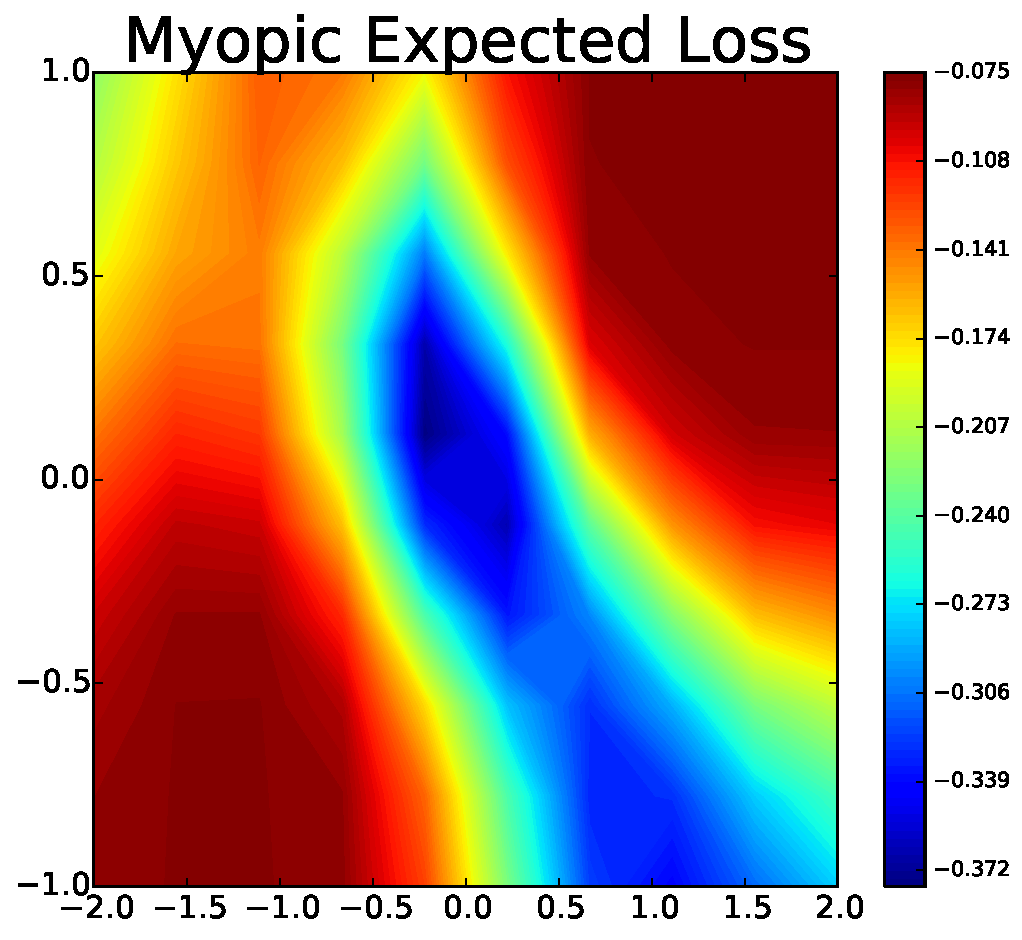
\includegraphics[width=54mm]{bo_1step.pdf}} &
      \addheight{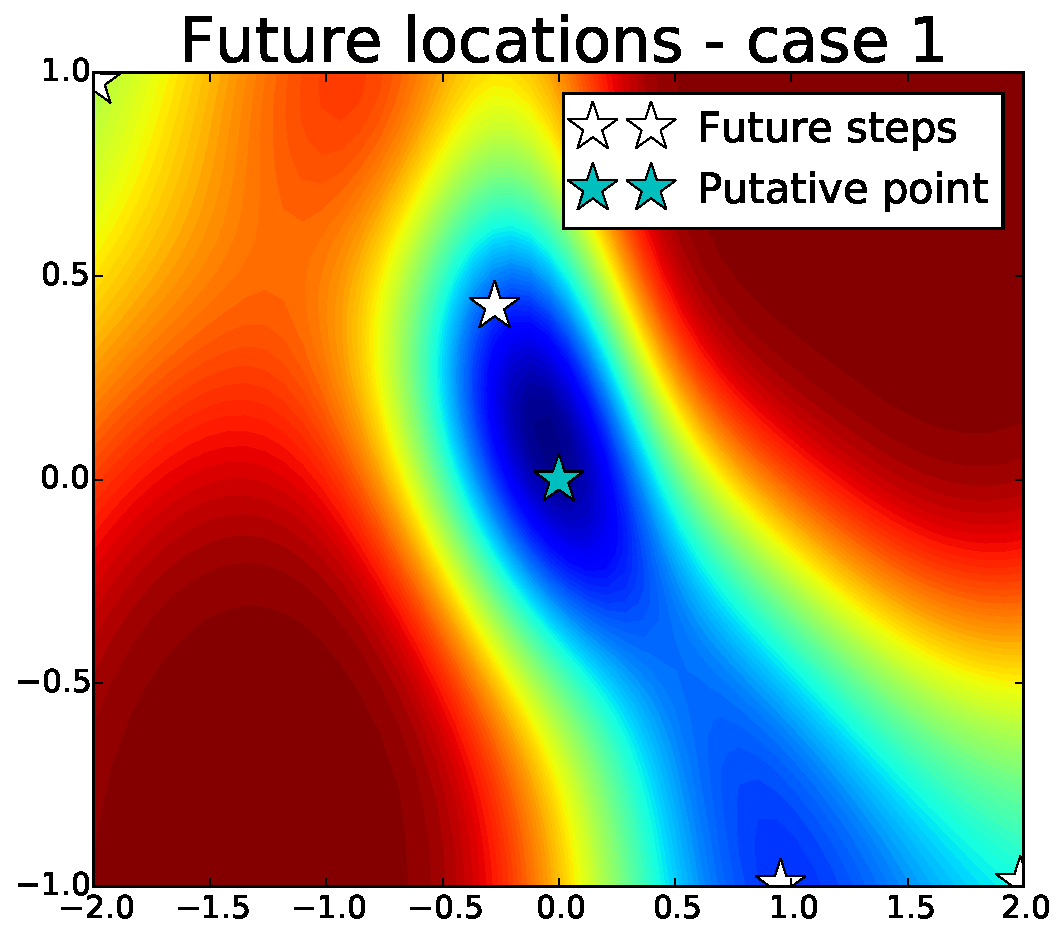
\includegraphics[width=54mm]{predicted_locations1.pdf}}  &
      \addheight{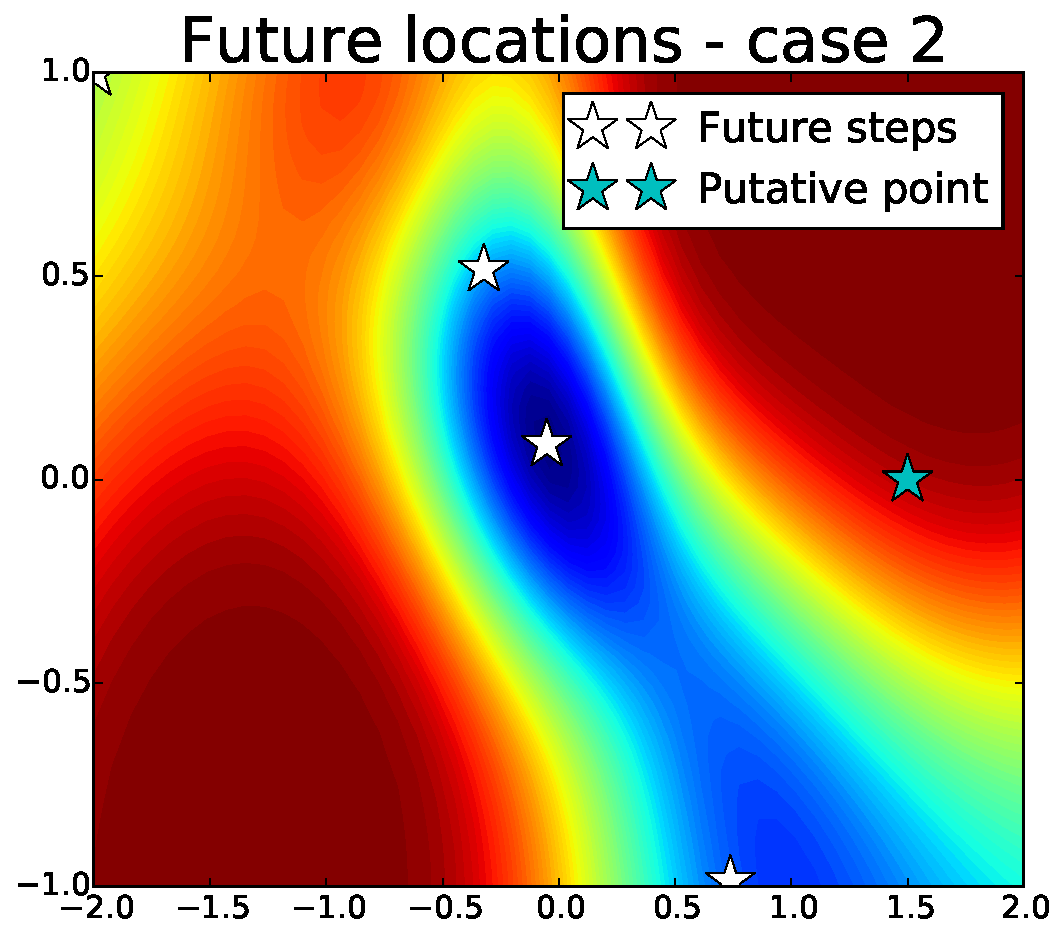
\includegraphics[width=54mm]{predicted_locations2.pdf}}\\
 %     \small Myopic loss &  \small 2 steps ahead & \small 3 steps ahead \\
\end{tabular}\caption{}
\end{table*}


\begin{figure*}[t!]
\begin{center}
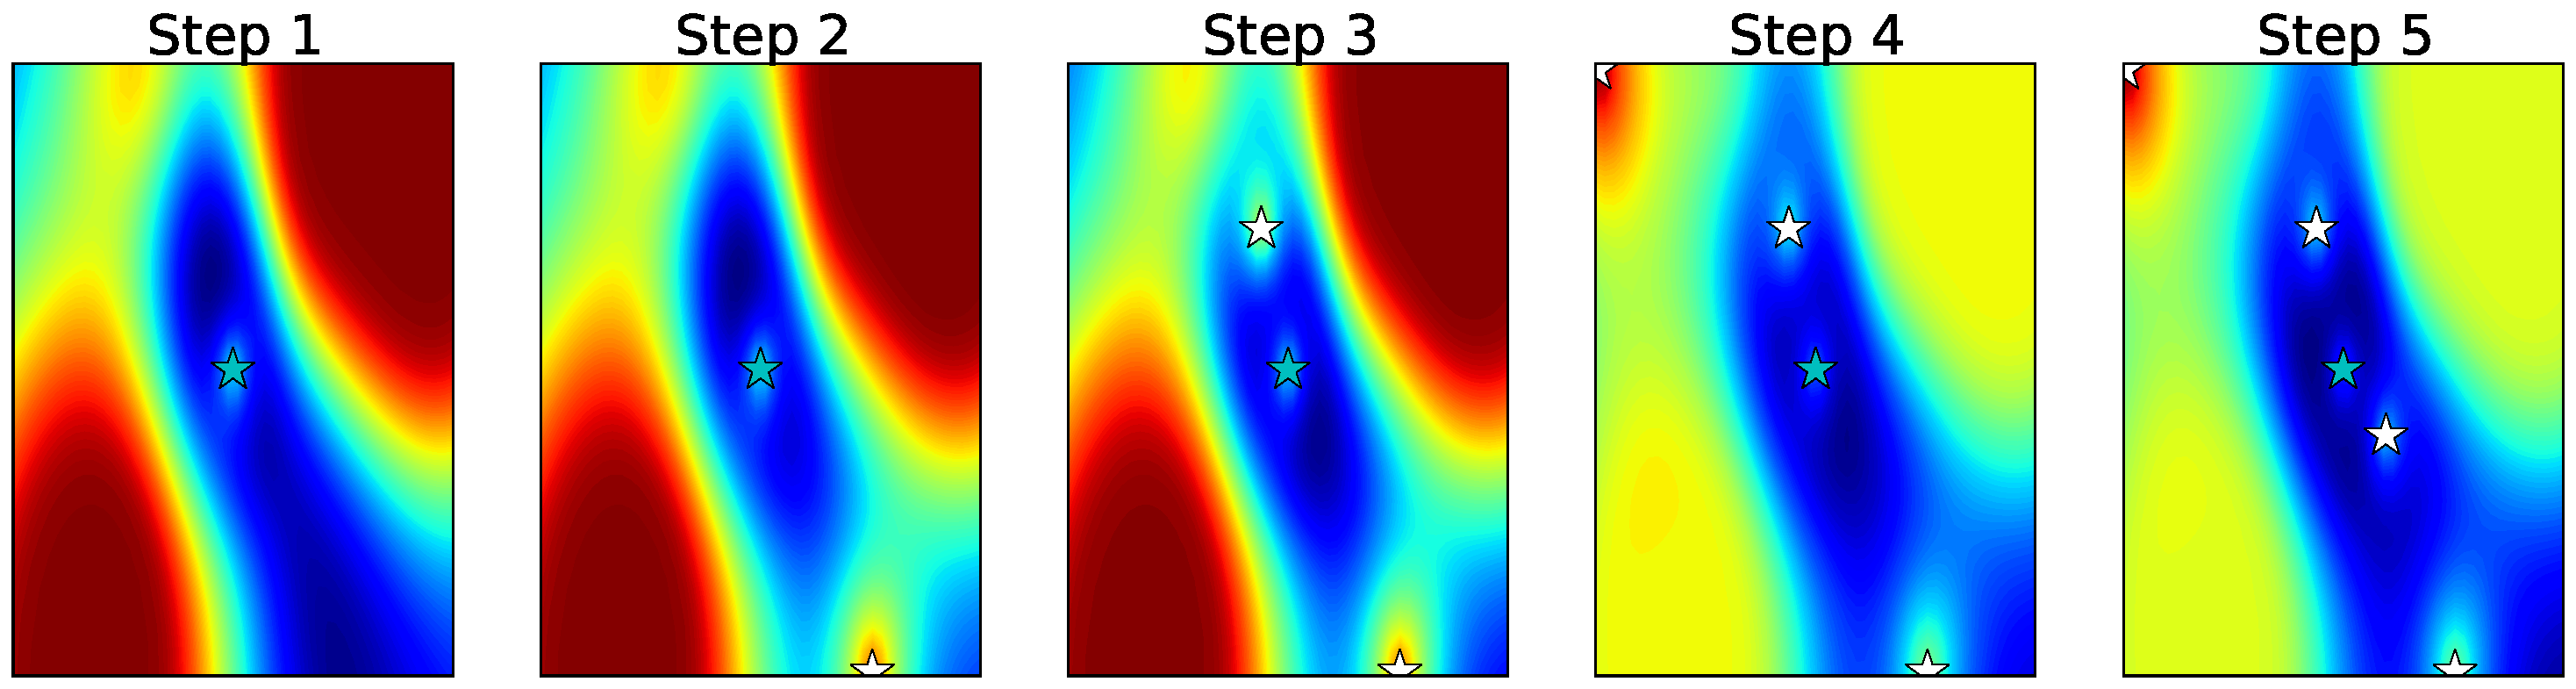
\includegraphics[width=16cm]{steps.pdf}
\end{center}\caption{ffff}
\end{figure*}

\begin{equation}\label{eq:penalized_acquisition}
 [\future_n(\bx_*)]_k  =\arg \max_{x \in \bx} \left\{g(\Lambda_1(\bx_*| \I_0))\prod_{j=1}^{k-1}\varphi(\bx;\hat{\bx}_{j})\right\},
\end{equation}
where $\varphi(\bx;\bx_{j})$ are local local penalizers centered at $\bx_{j}$ and $g:\bbbr \rightarrow \bbbr^+$  the \emph{soft-plus} transformation $g(z)= \ln(1+e^z)$ elsewhere.


\subsection{Algorithm and computational details}


\begin{algorithm*}[t!]
   \caption{Decision process of the \us algorithm.}
   \label{alg:glasses}
\begin{algorithmic}
   \STATE {\bfseries Input:} dataset $\mathcal{D}_{0} = \{(\textbf{x}_0, y_0)\}$, number of remaining evaluations ($n$), look-ahead predictor $\future$.
   \FOR{$j=0$ {\bfseries to} $n$ }
   \STATE 1. Fit a \gp with kernel $k$ to $\mathcal{D}_{j}$.
   \STATE 2. Build a predictor of the future $n-l$ evaluations: $\future_{n-j}(\bx_*)$.
   \STATE 3. Select next location $\bx_j$ by taking  $\bx_j = \arg \min_{\bx \in {\mathcal X}}\Lambda_{n-j}(\bx_*|\I_0, \future_{n-j}(\bx_*))$.
   \STATE 4. Evaluate $f$ at $\bx_j$ and obtain $y_j$.
   \STATE 5. Augment the dataset $\mathcal{D}_{j} = \{\mathcal{D}_{j-1} \cup (\textbf{x}_j, y_j)\}$.
   \ENDFOR
   \STATE \textbf{Returns}: New location at $\arg \min_{x \in \mathcal{X}} \left\{\mu_2(\bx)\right\}$.  
\end{algorithmic}
\end{algorithm*}

\section{Results}\label{sec:experiments}


\subsection{Testing the validity of the approach}
To study the validity of our approximation we choose a variety of functions with a range  of dimensions and domains domain sizes. See Table \ref{} for details.

\begin{table}[t!]
\begin{center}
\begin{tabular}{lcc}
\toprule
Name &Function domain & $D$ \\
\midrule
\hline
Cosines & $[0,1]\times[0,1]$ & 2\\
Branin &$[-5,10]\times[-5,10]$ & 2\\
 Sixhumpcamel  &$[-2,2]\times[-1,1]$ & 2\\
McCormick  & $[-1.5,4]\times[-3,4]$& 2\\
Goldstein &$[-2,2]\times[-2,2]$& 2\\
Egg-holder   &$[-512,512]\times[-512,512]$ & 2\\
Powers  & $[-1,1]\times[-1,1]$& 2\\ \hline
Alpine2-2  &  & 2\\
Alpine2-5  & $[-10,10]^{D}$& 5\\
Alpine2-10  & & 10\\\hline
gSobol-2  & & 2\\
gSobol-5  &$[-5,5]^{D}$ & 5\\
gSobol-10  & & 10\\
\bottomrule
\end{tabular}\caption{Details of the functions used in the experiments}
\end{center}
\end{table}


\begin{table*}[t!]
\begin{center}
\begin{tabular}{lrrrrrr}
\toprule
     noise-free &        EL &      GL-2 &      GL-3 &      GL-5 &     GL-10 & GL-(n-k) \\
\midrule
      Cosines & -1.562084 & -1.577403 & -1.586372 & \textbf{-1.600443} & -1.465383 &\\
       Branin &  \textbf{0.727696} &  1.018735 &  1.865223 &  1.847867 &  1.190992 & \\
 Sixhumpcamel & \textbf{-1.111226} & -1.099144 & -1.085236 & -1.091393 & -1.104145 & \\
    McCormick & -1.939604 & -1.936456 & -1.916778 & -1.950658 & \textbf{-2.003377} & \\
       Goldstein &&&&&\\
       Egg-holder &&&&&\\   
       Powers & -0.125614 & \textbf{-0.185978} & -0.149429 & -0.158541 & -0.180303 & \\
       Alpine2 (d=2) &&&&&\\
       Alpine2 (d=5) &&&&&\\
       Alpine2 (d=10) &&&&&\\
       gSobol (d=2) &&&&&\\
       gSobol (d=5) &&&&&\\
       gSobol (d=10) &&&&&\\
\bottomrule
\toprule
     $sd.=0.1 $ &        EL &      GL-2 &      GL-3 &      GL-5 &     GL-10 & GL-(n-k) \\
\midrule
      Cosines & -1.562084 & -1.577403 & -1.586372 & \textbf{-1.600443} & -1.465383 &\\
       Branin &  \textbf{0.727696} &  1.018735 &  1.865223 &  1.847867 &  1.190992 & \\
 Sixhumpcamel & \textbf{-1.111226} & -1.099144 & -1.085236 & -1.091393 & -1.104145 & \\
    McCormick & -1.939604 & -1.936456 & -1.916778 & -1.950658 & \textbf{-2.003377} & \\
       Powers & -0.125614 & \textbf{-0.185978} & -0.149429 & -0.158541 & -0.180303 & \\
              Goldstein &&&&&\\
       Egg-holder &&&&&\\   
       Alpine2 (d=2) &&&&&\\
       Alpine2 (d=5) &&&&&\\
       Alpine2 (d=10) &&&&&\\
       gSobol (d=2) &&&&&\\
       gSobol (d=5) &&&&&\\
       gSobol (d=10) &&&&&\\
\bottomrule
\end{tabular}\caption{Results for the mean of the replicates}
\end{center}
\end{table*}

%\begin{table*}
%\begin{tabular}{lrrrrr}
%\toprule
 %     problem &        EL &      GL-2 &      GL-3 &      GL-5 &     GL-10 \\
%\midrule
%      cosines & -1.641266 & -1.614421 & -1.647324 & \textbf{-1.685686} & -1.496753 \\
%       branin &  \textbf{0.501499} &  0.776298 &  1.223222 &  0.791490 &  0.626915 \\
% sixhumpcamel & \textbf{-1.115223} & -1.096584 & -1.073318 & -1.098454 & -1.103938 \\
%    mccormick & -1.970486 & -1.996537 & -1.966840 & -1.998333 & \textbf{-2.031038} \\
%       powers & -0.123350 & -0.159824 & -0.152354 & -0.125650 & \textbf{-0.172454} \\
%\bottomrule
%\end{tabular}\caption{Results for the median of the replicates}
%\end{table*}

%\begin{table*}
%\begin{tabular}{lrrrrr}
%\toprule
%      problem &        EL &      GL-2 &      GL-3 &      GL-5 &     GL-10 \\
%\midrule
%      cosines & -1.700992 & -1.899286 & -1.803843 & -1.815387 & \textbf{-1.935917} \\
%       branin &  0.395783 &  \textbf{0.282889} &  0.367038 &  0.305713 &  0.388108 \\
% sixhumpcamel & -1.225345 & -1.240747 & -1.170774 & -1.201114 & \textbf{-1.296890} \\
%    mccormick & \textbf{-2.128225} & -2.126073 & -2.038700 & -2.055372 & -2.077451 \\
%       powers & -0.184954 & \textbf{-0.350845} & -0.267484 & -0.287553 & -0.252537 \\
%\bottomrule
%\end{tabular}\caption{Results for the median of the replicates}
%\end{table*}

\section{Conclusions}\label{sec:conclusions}

\bibliographystyle{plainnat}
\bibliography{bib_glasses}

\newpage
\clearpage
\setcounter{section}{0}
\setcounter{equation}{0}
\renewcommand{\thesection}{S\arabic{section}}
\renewcommand{\theequation}{S.\arabic{equation}}
\onecolumn
\begin{center}
{\Large  \textbf{Supplementary materials for:\\
`GLASSES: Relieving The Myopia Of Bayesian Optimisation"}}
\end{center}
\begin{center}
\textbf{Authors here}
\end{center}

\vspace{1cm}
\section{Oracle Multiple Steps loook-ahead Expected Loss }
Denote by $\eta_n = \min \{\bY_0, y_*, y_2\dots,y_{n-1}\}$ the value of the best visited location when looking at $n$ evaluations in the future. Note that $\eta_n$ reduces to the current best lost $\eta$ in the one step-ahead case. It is straightforward to see that 
$$ \min (y_n,\eta_n) = \min (\by,\eta ).$$
It holds hat
\begin{eqnarray}\nonumber
\Lambda_n(\bx_*|\I_0, \future_{n}(\bx_*)) & = & \int \min (\by,\eta) \prod_{j=1}^{n}p(y_{j}|\I_{j-1}, \future_{n}(\bx_*)) \ud y_*\dots \ud y_n
\end{eqnarray}
where the integrals with respect to $\bx_2\dots \ud\bx_n$ are  $p(\bx_{j}|\I_{j-1}, \future_{n}(\bx_*))=1$, $j=2,\dots,n$ since we don't need to optimize for any location and $p(y_{j}|\bx_{j},\I_{j-1}, \future_{n}(\bx_*))=p(y_{j}|\I_{j-1}, \future_{n}(\bx_*))$. Notice that
\begin{eqnarray}\nonumber
\prod_{j=1}^{n}p(y_{j}|\I_{j-1}, \future_{n}(\bx_*))& =& p(y_n|\I_{n-1}, \future_{n}(\bx_*)) \prod_{j=1}^{n-1}p(y_{j}|\I_{j-1} \future_{n}(\bx_*))\\\nonumber
& = & p(y_n,y_{n-1}|\I_{n-2}, \future_{n}(\bx_*))  \prod_{j=1}^{n-2}p(y_{j}|\I_{j-1} \future_{n}(\bx_*))\\\nonumber
& & \dots \\\nonumber
& = & p(y_n,y_{n-1},\dots,y_2|\I_{1}, \future_{n}(\bx_*))\prod_{j=1}^{2}p(y_{j}|\I_{j-1} \future_{n}(\bx_*))\\\nonumber
& = & p(\by|\I_{0}, \future_{n}(\bx_*)) \nonumber
\end{eqnarray}
and therefore 
$$ \Lambda_n(\bx_*|\I_0, \future_{n}(\bx_*)) =\E [\min (\by,\eta)] =\int \min (\by,\eta)p(\by|\I_{0}, \future_{n}(\bx_*))d\by  $$

\vspace{1cm}
\section{Formulation of the Oracle Multiple Steps loook-ahead Expected Loss to be computed using Expectation Propagation}
Assume that $\by \sim \N(\by; \mu, \Sigma)$. Then we have that
\begin{eqnarray}\nonumber
\E[\min (\by,\eta)] & = & \int_{\IR^n} \min (\by,\eta)  \N(\by; \mu, \Sigma) d\by\\ \nonumber
& = & \int_{\IR^n - (\eta,\infty)^n } \min (\by)  \N(\by; \mu, \Sigma) d\by + \int_{(\eta,\infty)^n} \eta  \N(\by; \mu, \Sigma) d\by.  \nonumber
\end{eqnarray}
The first term can be written as follows:
\begin{equation}
 \int_{\IR^n - (\eta,\infty)^n } \min (\by)  \N(\by; \mu, \Sigma) d\by  =    \sum_{j=1}^n \int_{P_j} y_j \N(\by; \mu, \Sigma) \ud \by \nonumber
\end{equation}\nonumber
where $P_j := \{ \by \in\IR^n - (\eta,\infty)^n  : y_j \leq y_i,\,\, \forall i \neq j \}$. We can do this because the regions $P_j$ are disjoint and it holds that $\cup_{j=1}^{n}P_j = \IR^n - (\eta,\infty)^n $.  Also, note that the $\min(\by)$ can be replaced within the integrals since within each $P_j$ it holds that $\min(\by) = y_j$. Rewriting the integral in terms of indicator functions we have that
\begin{eqnarray}\label{eq:term1}
 \sum_{j=1}^n \int_{P_j} y_j \N(\by; \mu, \Sigma) \ud \by   =  \sum_{j=1}^n  \int_{\IR^n} y_j \prod_{i=1}^n t_{j,i}(\by) \N(\by; \mu, \Sigma) \ud \by 
\end{eqnarray}

where $t_{j,i}(y) =\mathbb{I}\{y_i \leq\eta\}$ if $j=i$ and $t_{j,i}(y) =\mathbb{I}\{y_j \leq y_i \}$ otherwise.

The second term can be written as
\begin{equation}\label{eq:term2}
 \int_{(\eta,\infty)^n } \eta  \N(\by; \mu, \Sigma) d\by = \eta\int_{\IR^n} \prod_{i=1}^nh_i(\by) \N(\by; \mu, \Sigma) d\by
\end{equation}
where $h_i(\by) = \mathbb{I}\{y_i>\eta\}$.  Merge (\ref{eq:term1}) and (\ref{eq:term2}) to obtain Eq.  (\ref{eq:expected_loss_oracle}).
 



\end{document}
